\clearemptydoublepage
\backmatter

\chapter*{Conclusion}
\addcontentsline{toc}{chapter}{Conclusion}
\chaptermark{Conclusion}
%What are my takeaways ? Future work ?
%Theoretical point of view: Elegance and power of taking a model that represents the true complexity of the input.
%Practical point of view: the need for theoretical guarantees sometimes offsetted by %the technical complexity of those results, there are important and significant work to be done on engineering to yield efficient result in practice (space seed field seems especially interesting) 

\iffalse
\newpage
\chapter*{The Cat and the Yarn}

Inspired by the book "Le chat au pays des nombres" by Ivar Ekeland and John O'brien which presents the Hilbert's paradox of the Grand Hotel in a kids book format, I decided (on my own time) to sketch a comic inspired by this thesis:
\vfill
\begin{center}
    \frame{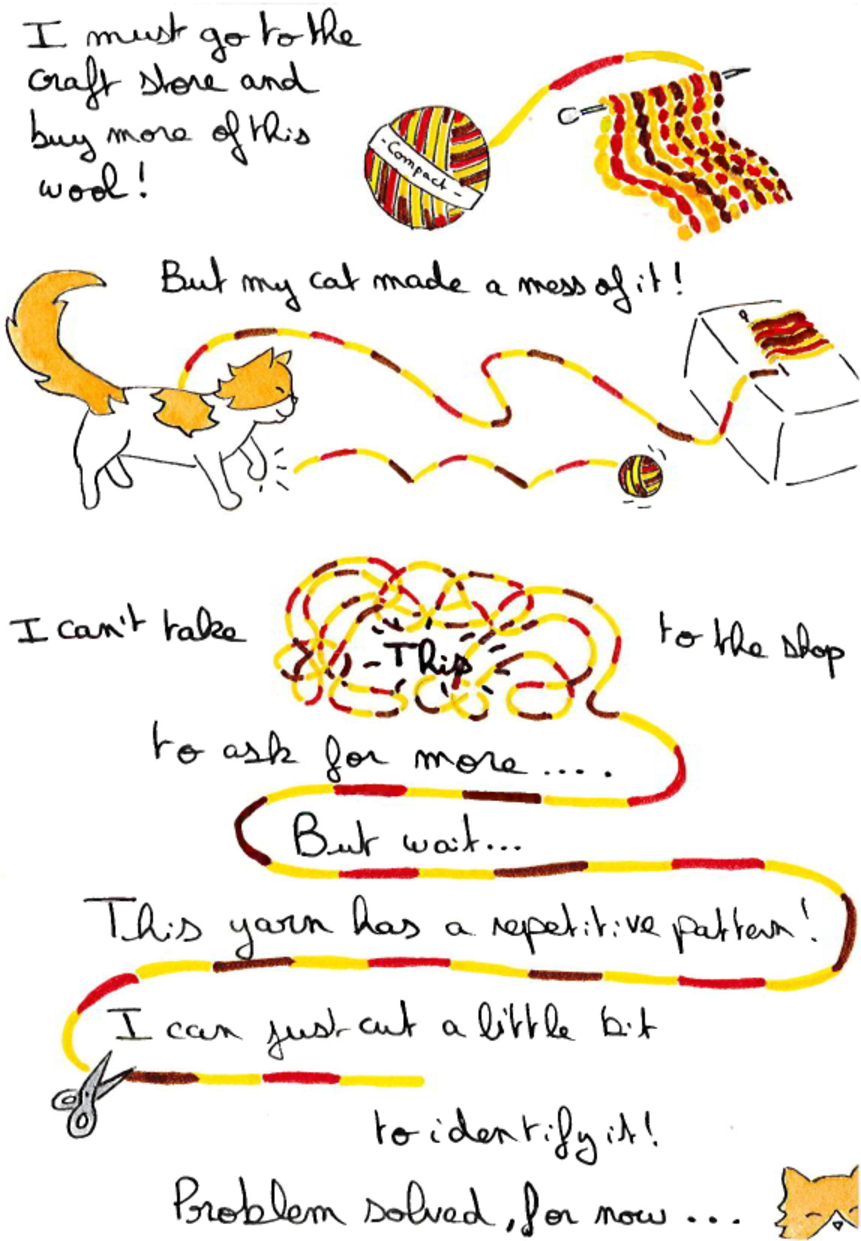
\includegraphics[width=12.5cm]{Conclusion/comic.pdf}}
\end{center}
\vfill
\fi